\chapter{Implementierung}\label{chap:Implementierung}
\thispagestyle{standard}
\pagestyle{standard}
\lfoot{\small Refik Kerimi}

In diesem Kapitel wird die Umsetzung der Applikation beschrieben.

\section{Anforderungsanalyse}\label{sub:Anforderungsanalyse}
Die zu entwickelnde Smart Home Applikation muss das Verhalten einer \acs{PWA} aufweisen. Das heißt es müssen die Attribute aus Kapitel \ref{chap:ProgressiveWebapplikationen} eingebaut werden und danach getestet werden siehe Kapitel \ref{chap:Funktionstest}. Außerdem sollen auch APIs entwickelt werden die es möglich machen mit Services von Drittanbietern die Temperatur zu regeln, mit Hilfe von Geolocation API den Standort zu ermitteln um das Garagentor über GPS automatisch öffnen zu können. Ebenso soll das Steuern der Beleuchtung möglich sein. Diese Applikation soll Offline so weit es geht verwendbar sein. Die Anwendung muss Plattformunabhängig und responsive sein.

\section{Umsetzung der Anforderungen}\label{sub:Umsetzung der Anforderungen}
Zur Umsetzung der Anforderungen aus Kapitel \ref{sub:Anforderungsanalyse} wurden für User Interface ReactJS\footnote{https://reactjs.org/docs/getting-started.html} und als CSS Framework Semantic-UI\footnote{https://react.semantic-ui.com/introduction} verwendet. Sematic-UI soll sicherstellen das die Applikation responsives Verhalten aufweist und für alle Bildschirmgrößen geeignet ist. Um die Daten zu versenden, aufzurufen und zu speichern wurde das JSON Key/Value Format, die Fetch API und der Browser Cache verwendet.
Als Browser diente der Google Chrome Browser Version 67.

\section{Ausgewählte Programmiersprache und IDE}
Als Programmiersprache wurde \acl{JS} (\acs{JS}) ausgewählt. 
Als Entwicklungsumgebung wurde Webstorm (Version 2018.2) von Jetbrains verwendet. 
Weitere verwendete Tools und Frameworks wurden in Kapitel \ref{sub:Umsetzung der Anforderungen} beschrieben.
\newpage
\section{Ordnerstruktur}
Die zwei wichtigsten Dateien befinden sich wie in Abbildung \ref{fig:OrdnerStrucktur} zu sehen ist, im App Verzeichnis.
Ebenfalls wichtig ist das app.js File das unter \textit{/app/src/js/app.js} zu finden ist.

\begin{figure}[h]
	\centering
	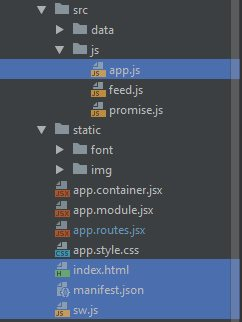
\includegraphics[width=10cm]{BilderAllgemein/Implementierung/OrdnerStrucktur.jpg}\medskip
	\caption{Ordner Struktur}
	\label{fig:OrdnerStrucktur}
\end{figure} 


\section{Manifest}
Das Manifest wird im Root Folder eingefügt und ist mit der Endung \acs{JSON} deklariert. Der genaue Pfad ist \textit{/app/manifest.json}. Wie in Kapitel \ref{sub:Manifest} schon beschrieben wurde, definiert das Manifest File das Aussehen des Icon am Startbildschirm, z.B. den Einstiegspunkt der App und den Namen. 
Die Listing \ref{lst:Manifest.json} zeigt weitere wichtige Eigenschaften:
\newpage
\begin{lstlisting}[language=json, firstnumber=1, caption={Manifest in das Projekt implementieren},label=lst:Manifest.json, xleftmargin=50pt]
{
  {
  "name":"PWA Smart Home",
  "short_name":"PWA_SHL_RMJ",
  "start_url":"./",
  "scope":".",
  "display":"standalone",
  "background_color":"#003399",
  "theme_color":"#3F51C5",
  "description":"Keep running with PWA",
  "dir":"ltr",
  "lang":"de-DE",
  "orientation":"portrait-primary",
  "icons":[
    {
      "src":"./static/img/light48.png",
      "type":"image/png",
      "sizes":"48x48"
    },
    {
      "src":"./static/img/light512.png",
      "type":"image/png",
      "sizes":"512x512"
    }
  ]
}
}
\end{lstlisting}
\clearpage
\section{Add to Homescreen}
Damit der Add to Homescreen Banner erscheint müssen die Bedingungen aus dem Kapitel \ref{sub:AddtoHomescreen}erfüllt werden.
Nach Erfüllung dieser Forderungen wird der beforeinstallprompt Event wie in Listing \ref{lst:AddtoHomescreen} aufgerufen und in die deferredPrompt variable gespeichert.

Verzeichnis: \textit{/app/src/js/app.js}

\begin{lstlisting}[language=JavaScript, firstnumber=1, caption={Add to Homescreen Funktion} ,label=lst:AddtoHomescreen, xleftmargin=50pt]
var deferredPrompt;

window.addEventListener('beforeinstallprompt', event => {
    event.preventDefault();
    deferredPrompt = event;
    return false;
});
%\end{lstlisting}

Diese Callbackfunktion wird in die \textit{app.js} Datei implementiert. 

\section{Service Worker und Cache API}
Das Herzstück der Applikation ist der im Kapitel \ref{chab:FeaturesundMerkmale} beschriebene Service Worker. Als erstes muss validiert werden, ob der Service Worker vom Browser unterstützt wird und danach kann dieser registriert, installiert und aktiviert werden.
In den folgenden Listings \ref{lst:Registrierung}, \ref{lst:Installation} und \ref{lst:Aktivierung} sind die Funktionen, die für den Service Worker von Bedeutung sind aufgeführt und die wichtigsten Teile beschrieben.

Verzeichnis: \textit{/app/src/js/app.js}

\begin{lstlisting}[language=JavaScript, firstnumber=1, caption={Registrierung Service Worker} ,label=lst:Registrierung , xleftmargin=50pt]
//Registrierung und Validierung vom Service Worker
if ('serviceWorker' in navigator && 'Notification' in window) {
    console.log('Service Worker and Notification is supported')
    navigator.serviceWorker.register('/sw.js')
        .then(reg => {
            console.log('Service worker registered!', reg);

        })
        .catch(err => console.log(err));
}
\end{lstlisting}

\clearpage
Die Registriermethode \textit{register()} bekommt als Parameter die Service Worker Datei mitgegeben.

Verzeichnis: \textit{/app/sw.js}

\begin{lstlisting}[language=JavaScript, firstnumber=1, caption={Installation Service Worker} ,label=lst:Installation, xleftmargin=50pt]
self.addEventListener('install', event => {
    console.log('[Service Worker] Installing Service Worker ....', event);
    event.waitUntil(
        caches.open(cacheName)
            .then(cache => {
                console.log('[Service Worker] Precaching App Frame');
                cache.addAll(filesToCache);
            })
    )
});
}
\end{lstlisting}

Nach dem erneuten Laden der Anwendung wird im Listing \ref{lst:Installation} der Installations Eventlistener aufgerufen. Dieser installiert den Service Worker und cached die angegebenen Dateien um die App offline verwenden zu können. 

Durch die Funktion \textit{waitUntil()} wird mit der Installation gewartet, bis die Dateien die dieser Funktion als Parameter mitgegeben wurden, gecacht wurden. Durch die Cachemethode \textit{cache.All()} werden alle angegeben Dateien aufgerufen und es müssen nicht alle Dateien einzeln eingeben werden.
Nach der Installation wird der Service Worker aktiviert und kann dann vom Browser verwendet werden.

Verzeichnis: \textit{/app/sw.js}

\begin{lstlisting}[language=JavaScript, firstnumber=1, caption={Aktivierung Service Worker} ,label=lst:Aktivierung, xleftmargin=50pt]
self.addEventListener('activate', event => {
    console.log('[Service Worker] Activating Service Worker ....', event);
    return self.clients.claim();
})
\end{lstlisting}

Durch die \textit{self.clients.claim()} Methode in Zeile 3 wird sichergestellt, dass der Service Worker nur installiert wird, wenn alle Bedingungen erfüllt wurden.

In der Callback-Funktion \textit{respondWith()} werden die Daten aufgerufen und die \\match-Methode überprüft ob die Daten sich im Cache befinden.
Um den Event aufzurufen werden Promises für asynchrone Aufrufe verwendet .
Um Daten aus dem Netzwerk aufzurufen die nicht im Cachespeicher vorhanden sind, wird über den fetch Event aufgerufen und überprüft wie in Abbildung \ref{lst:fetch} zu sehen.

Verzeichnis: \textit{/app/sw.js}

\begin{lstlisting}[language=JavaScript, firstnumber=1, caption={fetch Callbackfunktion} ,label=lst:fetch, xleftmargin=50pt]
self.addEventListener('fetch', event => {
    event.respondWith(
        caches.match(event.request)
            .then(response => {
                if (response) {
                    return response;
                }else{
                    return fetch(event.request);
                }
            })
    );
});
\end{lstlisting}


	 
\clearpage
\section{Offline Modus}
Eine der wichtigsten Aufgaben des Caches vom Service Worker ist der Offlinemodus oder das Arbeiten bei schlechter Internetverbindung. Der Cache beinhaltet im Grunde das Index.html File CSS und Bilder oder Icons. Bei der Entwicklung der Anwendung wurden statische Dateien wie im Listing \ref{lst:Cache} verwendet. Die benötigten Dateien wurden in die \textit{let fileToCache} Variable gespeichert und im Listing \ref{lst:Installation} und der \textit{caches.addAll()}-Methode als Parameter mitgegeben.


\begin{lstlisting}[language=JavaScript, firstnumber=1, caption={Cache} ,label=lst:Cache, xleftmargin=50pt]
let cacheName = 'precache';
let filesToCache = [
    '/',
    '/index.html',
    '/src/js/app.js',
    '/static/img/light48.png',
    '/static/img/dashboard-mockup.jpg',
    '/static/img/bulp.jpeg',
    '/static/img/garage.jpeg',
    '/static/img/Graph_Heizung.JPG',
    '/manifest.json'
];
\end{lstlisting}


\begin{figure}[H]
	\centering
	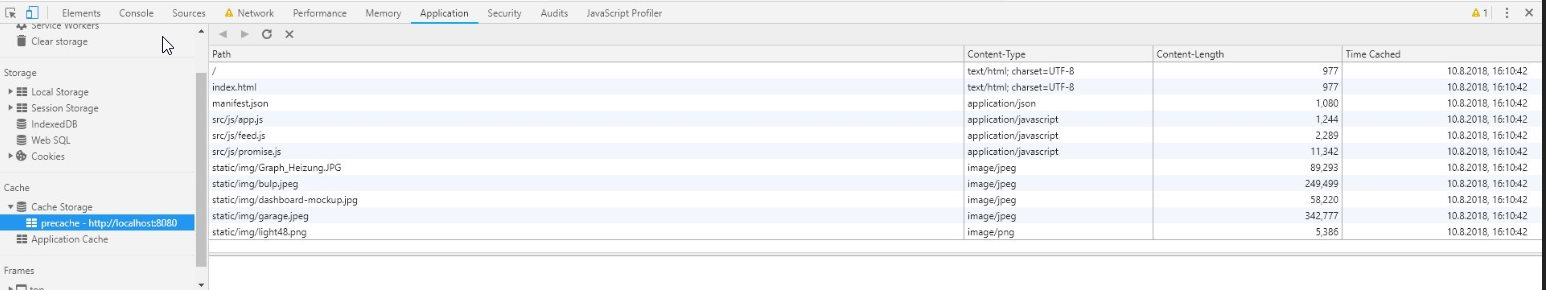
\includegraphics[width=16cm]{BilderAllgemein/Implementierung/Cache.jpg}\medskip
	\caption{Cache}
	\label{fig:Cache}
\end{figure}  

\begin{figure}[H]
	\centering
	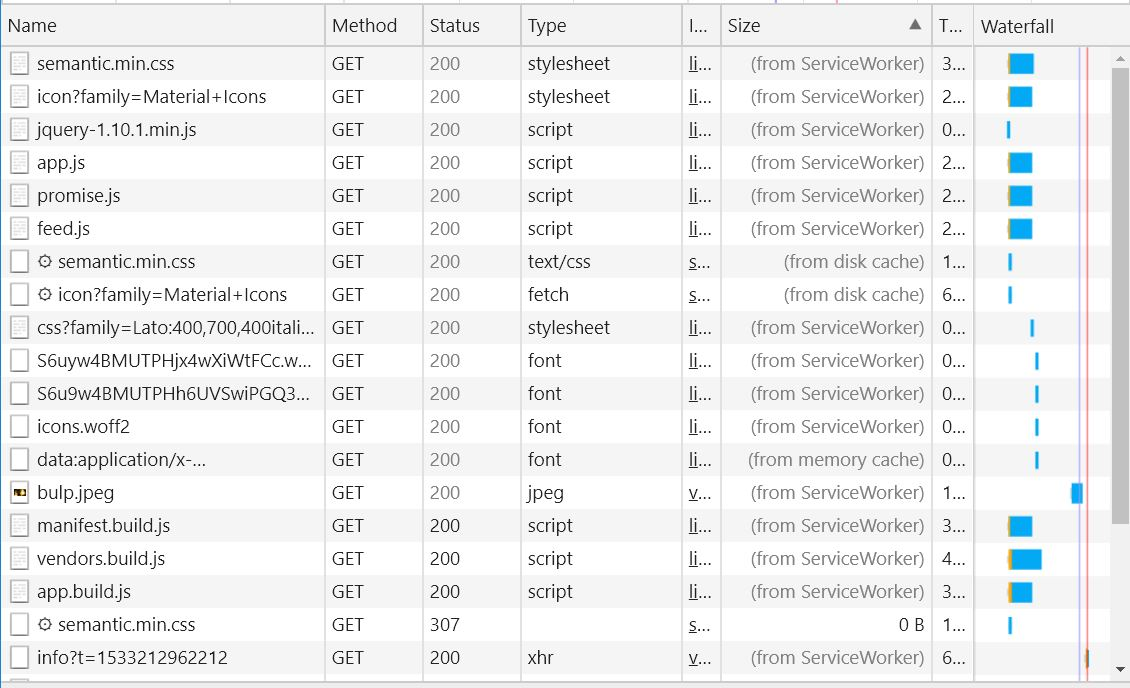
\includegraphics[width=8cm]{BilderAllgemein/Implementierung/aufruf_SW_Browser.jpg}\medskip
	\caption{Datenaufruf Service Worker}
	\label{fig:aufrufSWBrowser}
\end{figure}  

In der Abbildung \ref{fig:aufrufSWBrowser} und \ref{fig:Cache} sind die gecachten Files des Service Workers im Netzwerk und im Cache zu erkennen.



\clearpage
\section{Push Notifikation}
Die Push Benachrichtigungen dienen dem Nutzer dazu bei Änderungen im Haushalt benachrichtigt zu werden, z.B.: wenn das Licht defekt ist oder die Verbindung zur Heizung ausfällt.

Die Benachrichtigungen wurden in diesem Projekt nicht vom Server aus aufgerufen sondern sind über folgendes Listing im Pfad: \textit{/app/src/app.js} eingetragen. 
Nach der Überprüfung im Listing \ref{lst:Registrierung} ob die Pushfunktion im Browserscope vorhanden ist, wird in Listing \ref{lst:notificationsListener} der  Eventlistener über eine Callbackfunktion aufgerufen. Bei diesem Prototypen sind die Benachrichtigungen im JSON-File\\ (Verzeichnis: \textit{/app/src/data/notification.json}) und werden über eine fetch-API aufgerufen. Durch die \textit{openWindow()}-Funktion in Zeile 8 wird die Seite mit dem Benachrichtigungstext geöffnet.  
\\
\begin{lstlisting}[language=JavaScript, caption={Geolocation  Eventlistener} {\cite{PushNotifikationServer}},label=lst:notificationsListener, xleftmargin=50pt]
self.addEventListener('notificationclick', e => {
    let notification = e.notification;
    let action = e.action;

    if (action === 'close') {
        notification.close();
    } else {
        clients.openWindow('http://localhost:8080/benachrichtigungen');
        e.notification.close()

    }
});
\end{lstlisting}
\clearpage

\section{Geolocation API}
Um zu zeigen, dass der Zugriff auf die Geräte-APIs möglich ist, wurde in der Applikation eine Funktion hinzugefügt, die den genauen Standpunkt über die Geolocation-API ermittelt. Diese Funktion könnte als Garagenöffner oder zum Einschalten der Heizung nützlich sein. Wenn sich der Anwender dem Haus nähert, könnte über die GPS Daten das Tor geöffnet werden ohne, dass der Benutzer über eine HCI eingreifen muss. 
Als erstes wird im Listing \ref{lst:GeolocationSupport} der Support des Browsers überprüft.\\
Verzeichnis: \textit{/app/sw.js}

\begin{lstlisting}[language=JavaScript, caption={Geolocation  Support} {\cite{UserLocation}},label=lst:GeolocationSupport, xleftmargin=50pt]
if (navigator.geolocation) {
  console.log('Geolocation is supported!');
}
else {
  console.log('Geolocation is not supported for this Browser/OS.');
}
\end{lstlisting}

In der Abbildung \ref{fig:GeoSupport} sieht man, dass der Chrome Browser diese Geolocation Funktion unterstützt und man sieht auch die genauen Koordinaten.

\begin{figure}[h]
	\centering
	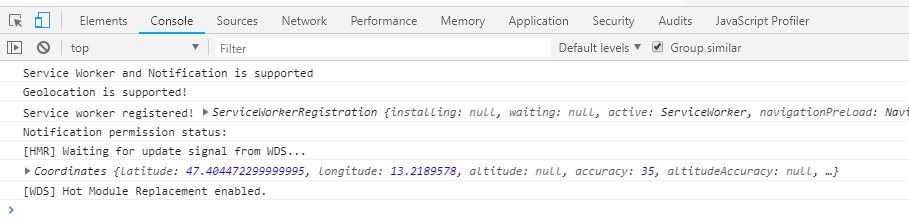
\includegraphics[width=14cm]{BilderAllgemein/Geolocation/GeoSupport.jpg}\medskip
	\caption{Konsolenmeldung Geolocation}
	\label{fig:GeoSupport}
\end{figure}







